\documentclass[10pt]{beamer}
\usetheme{metropolis}
\usepackage{booktabs}
\usepackage{tabularx}
\usepackage{calc}
\usepackage{tikz}
\usepackage{fontawesome5}
\usepackage{url}

% Setup for faculty images
\newlength{\imageheight}
\setlength{\imageheight}{3.5cm}

% Define CSUF brand colors
\definecolor{titanblue}{HTML}{00244E}
\definecolor{mediumblue}{HTML}{0F3F8C}
\definecolor{skyblue}{HTML}{EBFBFF}
\definecolor{titanorange}{HTML}{FF7900}
\definecolor{titangray}{HTML}{F5F5F5}
\definecolor{titantext}{HTML}{222222}

% Additional colors for the five environments
\definecolor{successcolor}{HTML}{27AE60}
\definecolor{warningcolor}{HTML}{F39C12}
\definecolor{dangercolor}{HTML}{E74C3C}

% Customize metropolis theme colors
\setbeamercolor{normal text}{fg=titantext, bg=white}
\setbeamercolor{alerted text}{fg=titanorange}
\setbeamercolor{example text}{fg=mediumblue}

% Title page colors
\setbeamercolor{title}{fg=titanblue, bg=white}
\setbeamercolor{subtitle}{fg=mediumblue, bg=white}
\setbeamercolor{institute}{fg=titanorange, bg=white}
\setbeamercolor{date}{fg=titanblue, bg=white}

% Frame title colors
\setbeamercolor{frametitle}{fg=white, bg=titanblue}
\setbeamercolor{framesubtitle}{fg=mediumblue, bg=white}

% Block environment colors
\setbeamercolor{block title}{fg=white, bg=titanblue}
\setbeamercolor{block body}{fg=titantext, bg=skyblue!10}

% Item colors
\setbeamercolor{itemize item}{fg=titanorange}
\setbeamercolor{itemize subitem}{fg=mediumblue}
\setbeamercolor{itemize subsubitem}{fg=titanblue}

% Footer and header colors
\setbeamercolor{footer}{fg=titantext}
\setbeamercolor{header}{fg=titanblue}

% Customize fonts
\setbeamerfont{title}{size=\Large, series=\bfseries}
\setbeamerfont{frametitle}{size=\large, series=\bfseries}

% Simple title page template
\defbeamertemplate*{title page}{customized}[1][]
{
\vspace{1cm}
 {\usebeamerfont{title}\usebeamercolor[fg]{title}\inserttitle\par}
\vspace{0.5cm}
 {\usebeamerfont{subtitle}\usebeamercolor[fg]{subtitle}\insertsubtitle\par}
\vspace{0.5cm}
 {\usebeamerfont{date}\usebeamercolor[fg]{date}\insertdate\par}
\vfill
 {\insertinstitute\par}
}

% Add progress bar
\makeatletter
\setbeamertemplate{headline}{%
\begin{beamercolorbox}[wd=\paperwidth,ht=0.4cm,dp=0cm]{titanblue}%
\begin{tikzpicture}
\fill[titanorange] (0,0) rectangle (\the\paperwidth*\insertframenumber/\inserttotalframenumber,0.4cm);
\end{tikzpicture}%
\end{beamercolorbox}%
}
\makeatother

\begin{document}

\title{The Policy Environment}
\subtitle{Understanding the Context of Policymaking\\POSC 315: Introduction to Public Policy\\Lecture 2 (Part 2 of 2)}
\date{Summer 2025}
\institute{California State University, Fullerton}

\maketitle

% Introduction
\begin{frame}
\frametitle{The Policy Environment}

\begin{block}{}
\centering
The policy environment is the context in which the policy process takes place and significantly influences policy decisions.
\end{block}

\pause
\vspace{0.5cm}
\textbf{Why Study the Policy Environment?}

To understand why certain policies are adopted while others are rejected, we must examine the broader context.

\end{frame}

% Overview of Environments
\begin{frame}
\frametitle{Components of the Policy Environment}

\begin{columns}
\begin{column}{0.18\textwidth}
\begin{block}{\textcolor{titanblue}{S}}
\pause
\centering
\textbf{Structural}

Political institutions and government structure
\end{block}
\end{column}

\begin{column}{0.18\textwidth}
\begin{block}{\textcolor{mediumblue}{S}}
\pause
\centering
\textbf{Social}

Demographics, culture, and social norms
\end{block}
\end{column}

\begin{column}{0.18\textwidth}
\begin{block}{\textcolor{successcolor}{E}}
\pause
\centering
\textbf{Economic}

Resources, markets, and financial conditions
\end{block}
\end{column}

\begin{column}{0.18\textwidth}
\begin{block}{\textcolor{warningcolor}{P}}
\pause
\centering
\textbf{Political}

Public opinion, elections, and political climate
\end{block}
\end{column}

\begin{column}{0.18\textwidth}
\begin{block}{\textcolor{dangercolor}{I}}
\pause
\centering
\textbf{International}

Global relationships and influences
\end{block}
\end{column}
\end{columns}

\pause
\vspace{0.5cm}
\centering
These environments interact with and influence each other

\end{frame}

% Structural Environment
\begin{frame}
\frametitle{The Structural Environment}

\begin{block}{}
The formal and informal political institutions that make and implement collective decisions.
\end{block}

\vspace{0.5cm}

\begin{columns}
\begin{column}{0.48\textwidth}
\begin{block}{Basic Features of American Government}
\pause
\begin{itemize}
\item Separation of powers
\item Federalism
\item Checks and balances
\end{itemize}
\end{block}
\end{column}

\begin{column}{0.48\textwidth}
\begin{block}{Policy Implications}
\pause
\begin{itemize}
\item Multiple points of access for influence
\item Difficulty passing major policies
\item Incremental change more common than radical reform
\end{itemize}
\end{block}
\end{column}
\end{columns}

\end{frame}

% Structural Constraints
\begin{frame}
\frametitle{Structural Constraints on Policy}

\begin{columns}
\begin{column}{0.32\textwidth}
\begin{block}{1. Constitutional}
\pause
The Constitution limits government power and protects certain rights
\end{block}
\end{column}

\begin{column}{0.32\textwidth}
\begin{block}{2. Institutional}
\pause
Established procedures and rules shape how policies are made
\end{block}
\end{column}

\begin{column}{0.32\textwidth}
\begin{block}{3. Jurisdictional}
\pause
Division of powers between federal, state, and local levels
\end{block}
\end{column}
\end{columns}

\end{frame}

% Social Environment
\begin{frame}
\frametitle{The Social Environment}

\begin{block}{Political Culture}
The set of shared beliefs, values, and norms that influence the political system.
\end{block}

\pause
\vspace{0.5cm}

\begin{block}{Basic Features of American Political Culture}
\begin{itemize}
\item Liberty
\item Equality
\item Democracy
\item Civic duty
\item Individual responsibility
\end{itemize}
\end{block}

\end{frame}

% Changing Demographics
\begin{frame}
\frametitle{Changing Demographics}

\begin{block}{The U.S. Population is Becoming:}
\end{block}

\begin{columns}
\begin{column}{0.48\textwidth}
\pause
\begin{itemize}
\item \textbf{More diverse}
\begin{itemize}
\item Racial and ethnic composition
\item Religious affiliation
\end{itemize}
\item \textbf{Older}
\begin{itemize}
\item Aging baby boomers
\item Longer life expectancy
\end{itemize}
\end{itemize}
\end{column}

\begin{column}{0.48\textwidth}
\pause
\begin{itemize}
\item \textbf{More urban}
\begin{itemize}
\item Rural to urban migration
\item Concentration in metropolitan areas
\end{itemize}
\item \textbf{More educated}
\begin{itemize}
\item Higher rates of college attendance
\item Increased specialized knowledge
\end{itemize}
\end{itemize}
\end{column}
\end{columns}

\pause
\vspace{0.5cm}
\centering
The government must respond to these changing needs through policy adaptation

\end{frame}

% Social Environment Policy Implications
\begin{frame}
\frametitle{Social Environment Policy Implications}

\begin{columns}
\begin{column}{0.48\textwidth}
\begin{block}{Challenges}
\pause
\begin{itemize}
\item Increasing demand for social services
\item Growing healthcare needs
\item Changing workforce dynamics
\item Housing and infrastructure pressures
\end{itemize}
\end{block}
\end{column}

\begin{column}{0.48\textwidth}
\begin{block}{Policy Responses}
\pause
\begin{itemize}
\item Social safety net programs
\item Healthcare reform efforts
\item Education and workforce development
\item Urban planning and development
\end{itemize}
\end{block}
\end{column}
\end{columns}

\end{frame}

% Economic Environment
\begin{frame}
\frametitle{The Economic Environment}

\begin{block}{Economic Conditions}
The state of the economy shapes policy priorities, options, and constraints.
\end{block}

\vspace{0.5cm}

\begin{columns}
\begin{column}{0.48\textwidth}
\begin{block}{Key Economic Factors}
\pause
\begin{itemize}
\item \textbf{Business cycle}
\begin{itemize}
\item Expansion $\rightarrow$ Peak $\rightarrow$ Contraction $\rightarrow$ Trough
\item Inflation and deflation
\item Unemployment
\item Economic growth
\item Income inequality
\end{itemize}
\end{itemize}
\end{block}
\end{column}

\begin{column}{0.48\textwidth}
\begin{block}{Economic Indicators}
\pause
\begin{itemize}
\item Gross Domestic Product (GDP)
\item GDP growth rate
\item Unemployment rate
\item Inflation rate (CPI)
\item Government debt and deficits
\item Poverty rate
\end{itemize}
\end{block}
\end{column}
\end{columns}

\end{frame}

% Political Environment
\begin{frame}
\frametitle{The Political Environment}

\begin{block}{National Mood}
The public's general attitude toward government and politics significantly influences policy development.
\end{block}

\vspace{0.5cm}

\begin{columns}
\begin{column}{0.48\textwidth}
\begin{block}{Measurement Tools}
\pause
\begin{itemize}
\item ``Direction of the Country'' polling
\item Presidential approval ratings
\item Congressional approval ratings
\item Trust in government metrics
\end{itemize}
\end{block}
\end{column}

\begin{column}{0.48\textwidth}
\begin{block}{Policy Implications}
\pause
\begin{itemize}
\item Window of opportunity for reforms
\item Constraints on unpopular initiatives
\item Electoral pressures on policymakers
\item Agenda-setting influence
\end{itemize}
\end{block}
\end{column}
\end{columns}

\end{frame}

% Most Important Problem
\begin{frame}
\frametitle{Most Important Problem}

\begin{block}{Public Priority Setting}
Gallup regularly asks: ``What do you think is the most important problem facing the country today?''
\end{block}

\pause
\vspace{0.5cm}

Responses to this question help identify public priorities and shape policy agendas

\vspace{1cm}

\centering
\small
Survey resources: \url{https://news.gallup.com/poll/1675/most-important-problem.aspx}

Analysis example: \textit{NYT 2016: The Most Important Problem Facing America?}

\end{frame}

% International Environment
\begin{frame}
\frametitle{The International Environment}

\begin{block}{Globalization}
\framesubtitle{The increasing interdependence of countries significantly impacts domestic policy decisions.}
\end{block}

\vspace{0.5cm}

\begin{columns}
\begin{column}{0.48\textwidth}
\begin{block}{Basic Features}
\pause
\begin{itemize}
\item \textbf{International economy}
\begin{itemize}
\item Trade agreements
\item Financial markets
\end{itemize}
\item \textbf{International organizations}
\begin{itemize}
\item UN, WTO, IMF, World Bank
\end{itemize}
\item International law and treaties
\end{itemize}
\end{block}
\end{column}

\begin{column}{0.48\textwidth}
\begin{block}{Policy Constraints}
\pause
\begin{itemize}
\item Trade obligations limit protectionist policies
\item Global competition affects labor/environmental standards
\item Treaty commitments require policy alignment
\item International pressure on human rights issues
\end{itemize}
\end{block}
\end{column}
\end{columns}

\end{frame}

% Integration of Environments
\begin{frame}
\frametitle{The Overall Policy Environment}

\begin{block}{}
The overall policy environment is the combination of the structural, social, economic, political, and international environments.
\end{block}

\pause
\vspace{0.5cm}

\begin{block}{Key Characteristics}
\begin{itemize}
\item The policy environment provides the context in which the policy process takes place
\item The policy environment influences what issues are considered, what options are available, and what solutions are implemented
\item The policy environment can enable or constrain policy choices
\item Different policy areas are affected by different aspects of the environment
\end{itemize}
\end{block}

\end{frame}

% Environment Interactions
\begin{frame}
\frametitle{Environment Interactions}

\begin{center}
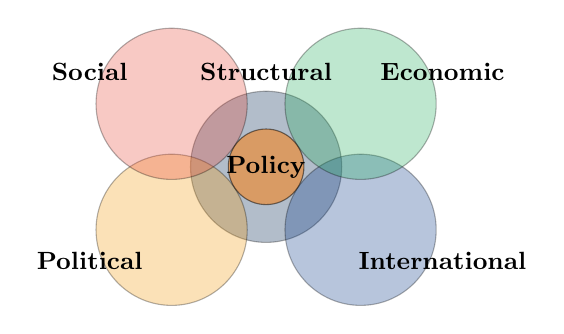
\begin{tikzpicture}[scale=0.8]
% Draw overlapping circles for each environment
\draw[fill=titanblue, opacity=0.3] (0,2) circle (1.2cm);
\draw[fill=mediumblue, opacity=0.3] (1.5,1) circle (1.2cm);
\draw[fill=successcolor, opacity=0.3] (1.5,3) circle (1.2cm);
\draw[fill=warningcolor, opacity=0.3] (-1.5,1) circle (1.2cm);
\draw[fill=dangercolor, opacity=0.3] (-1.5,3) circle (1.2cm);

% Central policy area
\draw[fill=titanorange, opacity=0.5] (0,2) circle (0.6cm);

% Labels
\node at (0,3.5) {\small \textbf{Structural}};
\node at (-2.8,3.5) {\small \textbf{Social}};
\node at (2.8,3.5) {\small \textbf{Economic}};
\node at (-2.8,0.5) {\small \textbf{Political}};
\node at (2.8,0.5) {\small \textbf{International}};
\node at (0,2) {\small \textbf{Policy}};
\end{tikzpicture}
\end{center}

\vspace{0.5cm}
\centering
Policy is shaped by the interaction of multiple overlapping environments

\end{frame}

% Case Study
\begin{frame}
\frametitle{Case Study: Healthcare Policy}
\framesubtitle{How different environmental factors influence healthcare policy in the U.S.}

\begin{columns}
\begin{column}{0.32\textwidth}
\begin{block}{Structural}
\begin{itemize}
\item Federalism divides responsibility
\item Constitutional questions about mandates
\item State vs. federal jurisdiction
\end{itemize}
\end{block}
\end{column}

\begin{column}{0.32\textwidth}
\begin{block}{Social \& Economic}
\begin{itemize}
\item Aging population
\item Rising costs
\item Employment-based insurance system
\end{itemize}
\end{block}
\end{column}

\begin{column}{0.32\textwidth}
\begin{block}{Political \& International}
\begin{itemize}
\item Ideological divisions
\item Interest group influence
\item Comparisons to other nations' systems
\end{itemize}
\end{block}
\end{column}
\end{columns}

\end{frame}

% Key Takeaways
\begin{frame}
\frametitle{Key Takeaways}

\begin{block}{}
\begin{itemize}
\item \textbf{Multiple Environments}: Policy is shaped by structural, social, economic, political, and international contexts
\item \textbf{Constraints and Opportunities}: Environments both limit and enable policy choices
\item \textbf{Interactions}: Environmental factors influence and reinforce each other
\item \textbf{Dynamic Nature}: Policy environments change over time, creating new challenges and opportunities
\item \textbf{Comprehensive Analysis}: Understanding the full environment is essential for effective policy analysis
\end{itemize}
\end{block}

\end{frame}

% Conclusion
\begin{frame}
\frametitle{That's it for Today!}
\framesubtitle{Remember to read Chapter Three for next time!}

\begin{block}{Review Questions}
\begin{itemize}
\item How do the stages and systems models help us understand the policy process?
\item Which environmental factors are most influential in your area of policy interest?
\item How might changes in one environment affect the others?
\end{itemize}
\end{block}

\end{frame}

\end{document}